
\begin{figure}[h!]
    \centering
        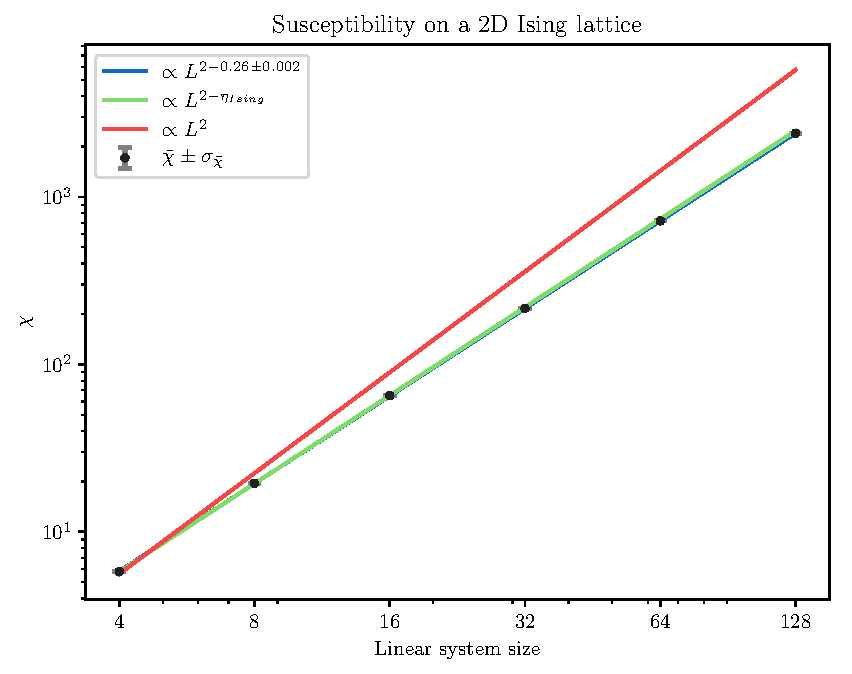
\includegraphics[width=0.8\textwidth]{figures/susceptibility128x128Ising.pdf}
    \caption{Scaling of susceptibility at $T_c$ on an Ising lattice of varying sizes. The measured critical exponent $\eta = 0.26 \pm 0.002$ is compared to the theoretical value $\eta_{Ising} = 0.25$ \cite{Plischke:EqStatMech}. The red line labeled $\propto L^2$ illustrates data where susceptibility scales with system size.}
    \label{fig:results_isingsusc}
\end{figure}

\begin{figure}[h!]
    \centering
        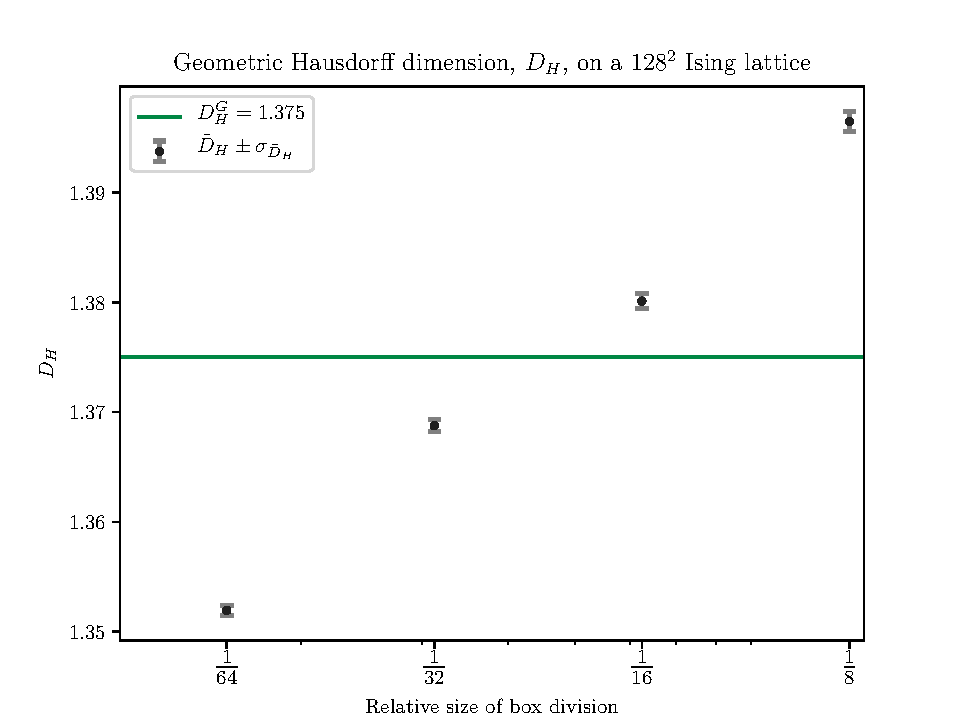
\includegraphics[width=0.8\textwidth]{figures/box_dim_128x128Ising.pdf}
    \caption{Hausdorff dimension of the maximum loop length on a $128^2$ Ising lattice at $T_c$ using the box dimension. The $x$ axis shows the size of one box relative to the side length of the lattice. The green line indicates the theoretical dimension of the geometric Ising cluster, $D_H^G = 1.375$ \cite{Duplantier:GeoHausdorff}. Comparing to the smallest box size as $D_H = 1.35193 \pm 5 \cdot 10^{-4}$.}
    \label{fig:results_boxdimension}
\end{figure}

\begin{figure}[h!]
    \centering
        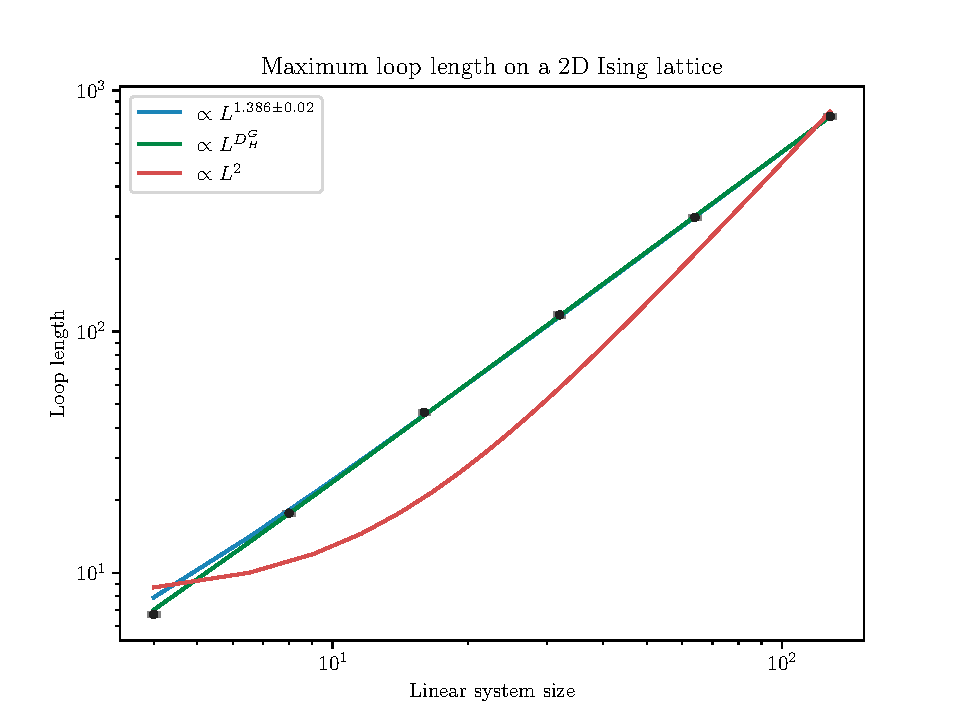
\includegraphics[width=0.8\textwidth]{figures/maximum_loop_length_for_2D_Ising.pdf}
    \caption{Log-log plot of the maximum loop length at $T_c$ on an Ising lattice of varying sizes. The measured scaling factor is $1.38 \pm 0.02$ compared to the theoretical Hausdorff dimension, $D_H^G = 1.375$ \cite{Duplantier:GeoHausdorff}. The red line labeled $\propto L^2$ illustrates data where maximum loop length scales with system size.}
    \label{fig:results_maxloopdimension}
\end{figure}


\begin{figure}[h!]
    \centering
        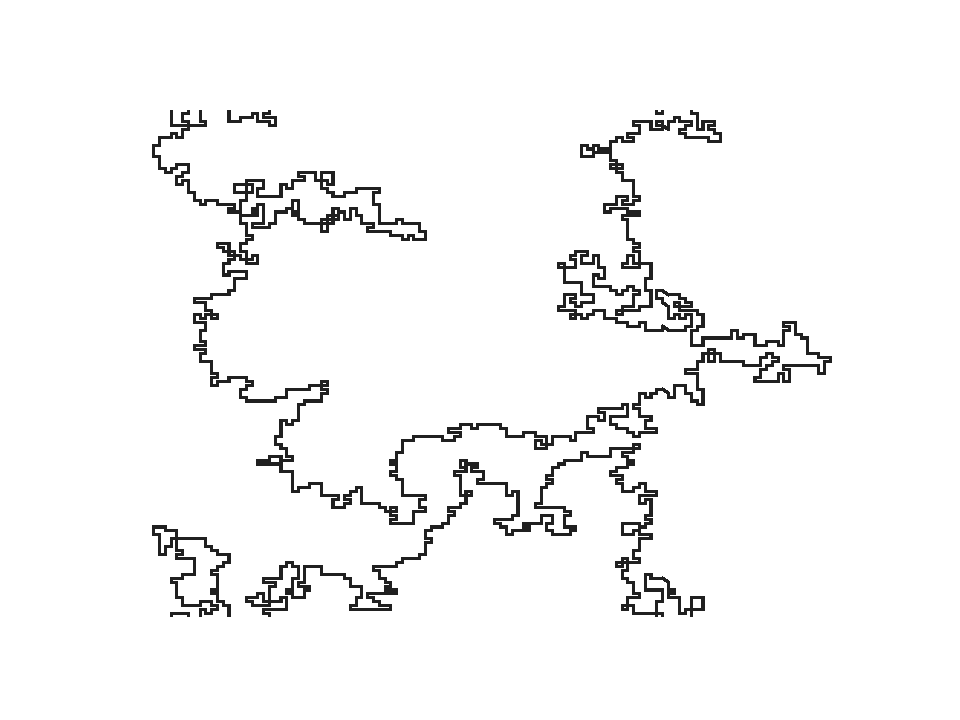
\includegraphics[width=0.8\textwidth]{figures/largest_cluster_testing_nolattice.pdf}
    \caption{Isolated largest cluster on a $128^2$ Ising lattice with periodic boundary conditions.}
    \label{fig:largest_cluster_illu}
\end{figure}

\begin{figure}[h!]
    \centering
        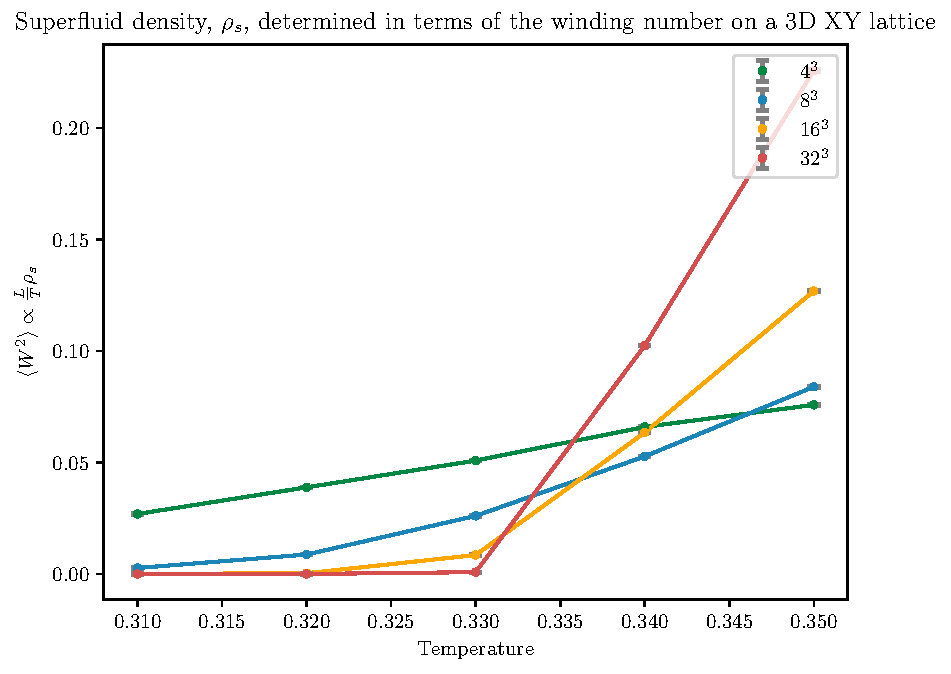
\includegraphics[width=0.8\textwidth]{figures/winding_number_Tc.pdf}
    \caption{Average winding number squared, $\langle W^2 \rangle \propto \rho_s$, plotted on a 3D XY lattice of varying sizes. The overall structure of the average winding number squared as a function of the temperature is shown.}
    \label{fig:results_windingnumberTc}
\end{figure}


\begin{figure}[h!]
    \centering
        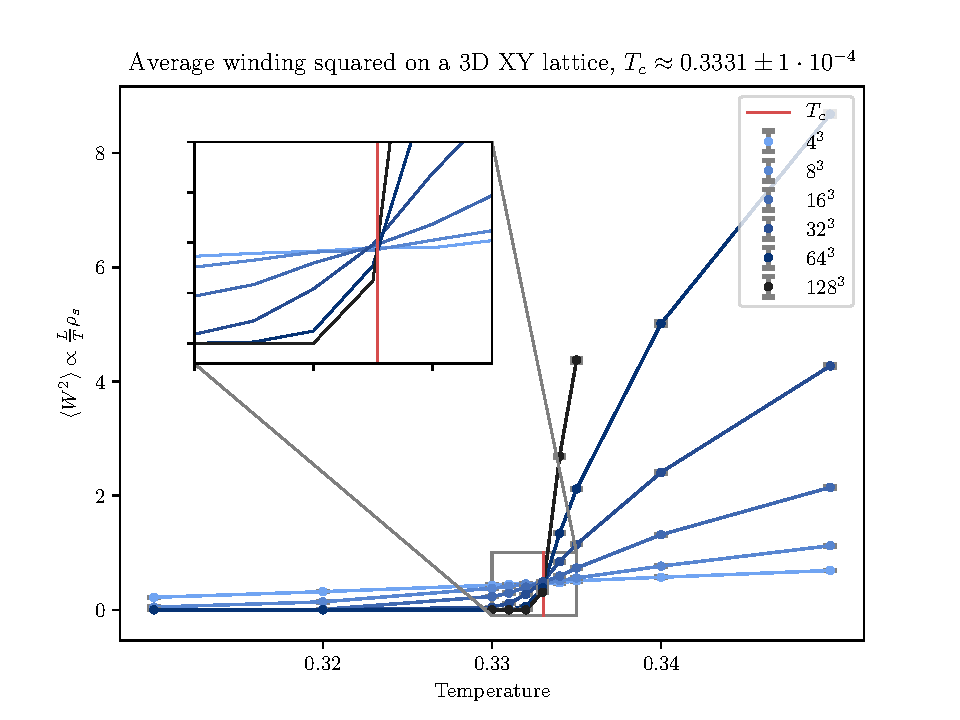
\includegraphics[width=0.8\textwidth]{figures/winding_number_Tc_zoomed.pdf}
    \caption{Average winding number squared, $\langle W^2 \rangle \propto \rho_s$, plotted on a 3D XY lattice of varying sizes. Due to the Villain approximation the transition is flipped such that $\rho_s \neq 0$ for $T > T_c$, and $T_c$ is translated from $\approx 2.2$ \cite{Gottlob:CritBehaviour3DXY} to $\approx 0.333$ indicated by the intersection. By taking the weighted average of the intersections the critical temperature can be estimated to $T_c = 0.3331 \pm 1 \cdot 10^{-4}$.}
    \label{fig:results_windingnumberTcZoomed}
\end{figure}

\begin{figure}[h!]
    \centering
        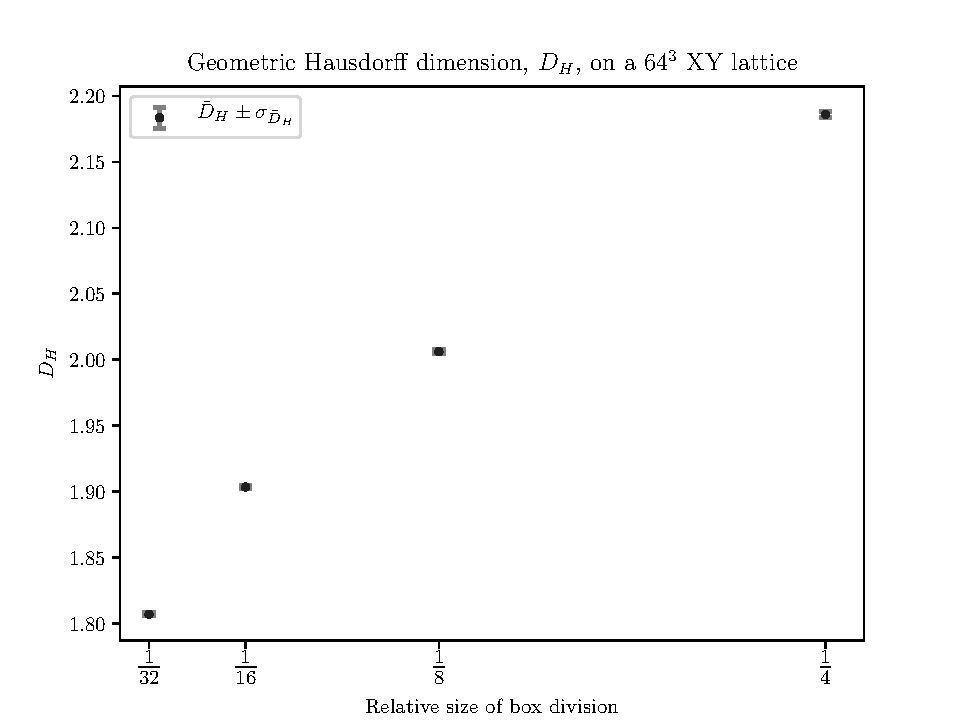
\includegraphics[width=0.8\textwidth]{figures/box_dim_64x64x64xy.pdf}
    \caption{Hausdorff dimension of the maximum loop length on a $64^3$ XY lattice at $T_c$ using the box dimension. The $x$ axis shows the size of one box relative to the side length of the lattice. Assuming that the smallest box size gives the best approximation, the result is $D_H = 1.807 \pm 5 \cdot 10^{-6}$.}
    \label{fig:results_boxdimension}
\end{figure}


\begin{figure}[h!]
    \centering
        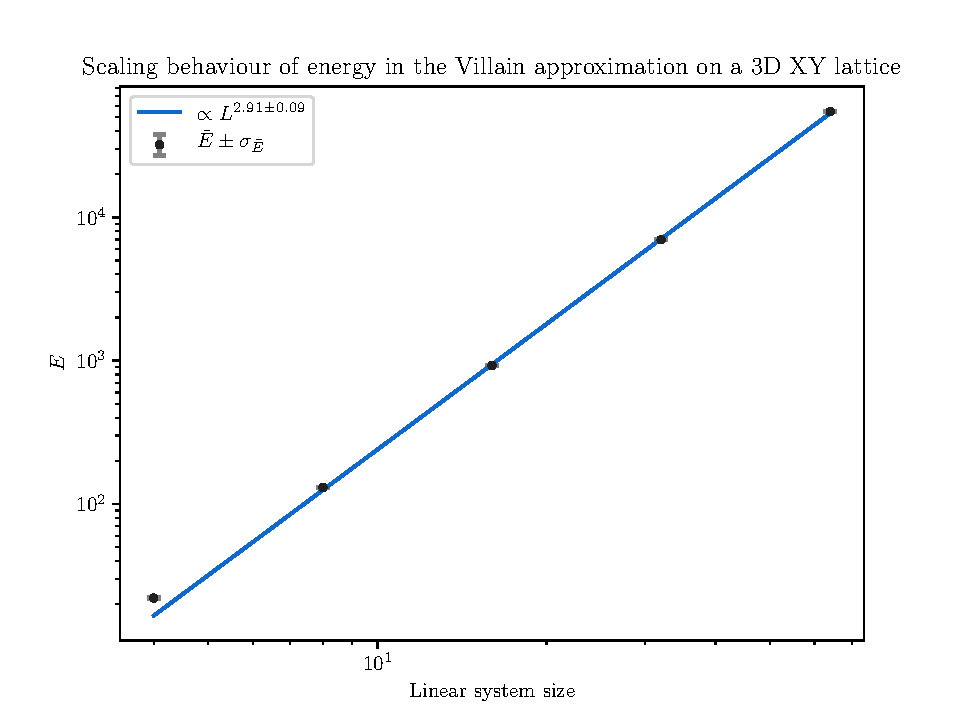
\includegraphics[width=0.8\textwidth]{figures/energy_scaling_xy.pdf}
    \caption{Log-log plot of the energy at $T_c$ on an 3D XY lattice of varying sizes. The measured scaling factor is $2.91 \pm 0.09$. The energy in the Villain approximation is proportional to the sum of the squares of flux flowing through the lattice.}
    \label{fig:results_energyxy}
\end{figure}

